\section{O papel do analisador sintático}

\begin{frame}[fragile]{Gramáticas no projeto de linguagens e na escrita de compiladores}

    \begin{itemize}
        \item Uma gramática oferece uma especificação sintática precisa para uma linguagem de programação
       %\pause

        \item Para certas classes de gramática é possível gerar o analisador sintático automaticamente
       %\pause

        \item O processo de construção do analisador sintático permite identificar ambiguidades sintáticas e outras construções difíceis de analisar, ajudando o
            projeto inicial de uma linguagem
       %\pause

        \item Uma gramática bem projetada implica uma estrutura na linguagem que é útil para a tradução para a linguagem alvo e para a detecção de erros
       %\pause

        \item A inclusão de novas características em uma linguagem é facilitada se a implementação foi baseada em uma descrição gramatical
    \end{itemize}

\end{frame}

\begin{frame}[fragile]{O papel do analisador sintático}

    \begin{itemize}
        \item O analisador sintático recebe, do analisador léxico, uma cadeia de \textit{tokens} e verifica se esta cadeia pode ser gerada pela gramática da
            linguagem-fonte
       %\pause

        \item Ele também deve relatar quaisquer erros de sintaxe que possam surgir, de forma inteligível
       %\pause

        \item Se possível, ele deve se recuperar dos erros mais comuns
       %\pause

        \item Ele pode produzir, explicitamente ou implicitamente, uma árvore sintática 
    \end{itemize}

\end{frame}

\begin{frame}[fragile]{Posição do analisador sintático num modelo de compilador}

    \begin{figure}
        \centering 

        \begin{scriptsize}
        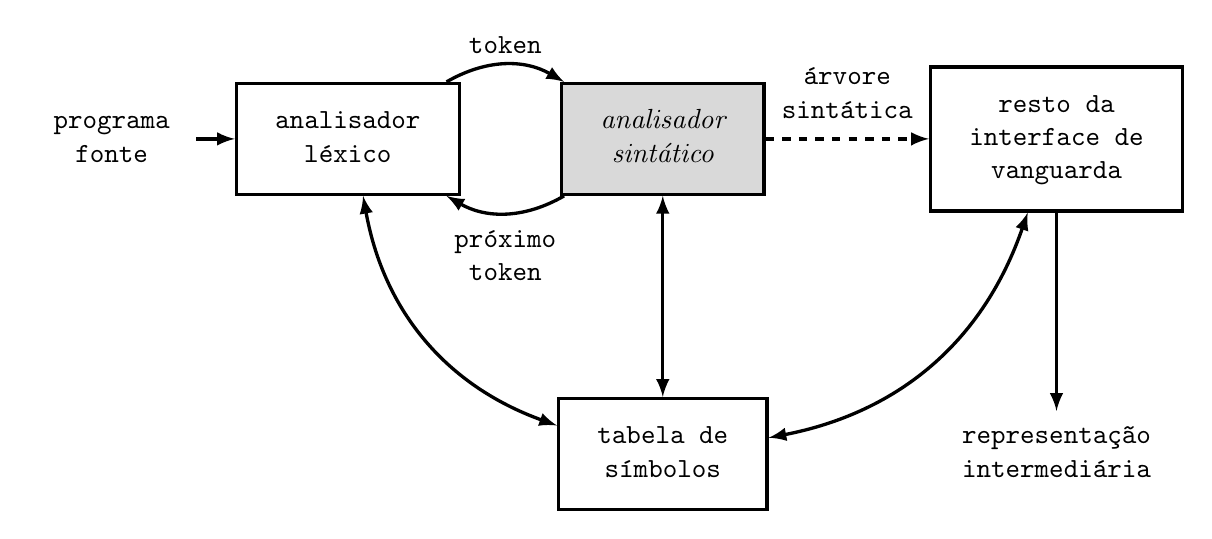
\begin{tikzpicture}
            \node (A) at (0, 6) { \texttt{\begin{tabular}{c}programa\\ fonte\end{tabular}} };
            \node[draw,very thick,inner sep=8pt] (B) at (3, 6) { \texttt{\begin{tabular}{c}analisador\\ léxico\end{tabular}} };
            \node[draw,very thick,inner sep=8pt,fill=gray!30] (C) at (7, 6) { \textit{\begin{tabular}{c}analisador\\ sintático\end{tabular}} };
            \node[draw,very thick,inner sep=8pt] (D) at (7, 2) { \texttt{\begin{tabular}{c}tabela de\\ símbolos\end{tabular}} };
            \node[draw,very thick,inner sep=8pt] (E) at (12, 6) { \texttt{\begin{tabular}{c}resto da\\ interface de\\ vanguarda\end{tabular}} };
            \node (F) at (12, 2) { \texttt{\begin{tabular}{c}representação\\ intermediária\end{tabular}} };

            \draw[very thick,-latex] (A) to (B);
            \draw[very thick,-latex] (B) to [bend left] node[above] { \texttt{token}} (C);
            \draw[very thick,-latex] (C) to [bend left] node[below] { \texttt{\begin{tabular}{c}próximo\\ token\end{tabular}}} (B);
            \draw[very thick,-latex,dashed] (C) to node[above] { \texttt{\begin{tabular}{c}árvore\\ sintática\end{tabular}} } (E);
            \draw[very thick,latex-latex] (B) to [bend right] (D);
            \draw[very thick,latex-latex] (E) to [bend left] (D);
            \draw[very thick,latex-latex] (C) to (D);
            \draw[very thick,-latex] (E) to (F);
        \end{tikzpicture}
        \end{scriptsize}
    \end{figure}

\end{frame}

\begin{frame}[fragile]{Tipos de analisadores sintáticos}

    \begin{itemize}
        \item Há três tipos gerais de analisadores sintáticos
       %\pause

        \item O primeiro tipo são os métodos universais, que podem tratar quaisquer gramáticas
       %\pause

        \item Exemplos de métodos gerais: o algoritmo de Younger-Kasami e o algoritmo de Early
       %\pause

        \item Tais métodos são ineficientes para um compilador de produção
       %\pause

        \item Os outros dois tipos são os analisadores \textit{top-down} e os analisadores \textit{bottom-up}
       %\pause

        \item Estes métodos trabalham apenas com uma determinada subclasse de gramáticas, porém são mais eficientes que os métodos universais
    \end{itemize}

\end{frame}

\begin{frame}[fragile]{Tipos de erro que um compilador pode encontrar}

    Dentre os diferentes tipos de erro que um compilador podem encontrar, há quatro importantes tipos de erro:
   %\pause

    \vspace{0.1in}

    \begin{enumerate}
        \item erros léxicos, relacionados aos tipos e a identificação dos tokens
       %\pause

        \item erros sintáticos, que surgem da inconformidade da disposição dos tokens em relação às regras gramaticais
       %\pause

        \item erros semânticos, que lidam com questões de compatibilidade de tipos e o significado das expressões da linguagem
       %\pause

        \item erros lógicos, que envolvem expressões semanticamente corretas mas que podem levar a laços infinitos e outros erros
    \end{enumerate}

\end{frame}

\begin{frame}[fragile]{Metas de um tratador de erros sintáticos}

    Há três metas principais a serem atingidas por um tratador de erros sintáticos:
   %\pause

    \vspace{0.1in}

    \begin{enumerate}
        \item Relatar a presença de erros de forma clara e precisa
       %\pause

        \item Recuperar-se de cada erro o mais rápido possível e de forma que se possa identificar os erros subsequentes
       %\pause

        \item Não atrasar o processamento de programas sintaticamente corretos
    \end{enumerate}
   %\pause

    \vspace{0.1in}
    Cada uma destas metas representa um desafio à parte.
\end{frame}

\begin{frame}[fragile]{Relato de erros}

    \begin{itemize}
        \item Uma vez encontrado um erro, o tratador deve produzir um relato (saída) que indique a natureza e a localização do erro no programa-fonte
       %\pause

        \item Em geral, o erro acontece no próprio token, ou alguns tokens antes, do token que está sendo avaliado quando o erro é identificado
       %\pause

        \item Uma estratégia simples é reportar a linha do programa-fonte onde se encontra o token em questão
       %\pause

        \item Se for possível identificar a natureza do erro, deve ser produzida uma mensagem compreensível sobre o erro e uma possível sugestão de
            correção
    \end{itemize}

\end{frame}

\begin{frame}[fragile]{Exemplo de código C++ com erro e a mensagem produzida pelo GCC}
    \inputsnippet{cpp}{1}{18}{codes/erro.cpp}
    \vspace{0.2in}
    \inputsnippet{bash}{1}{18}{codes/gcc.sh}
\end{frame}

\begin{frame}[fragile]{Estratégias de recuperação de erros}

    \begin{itemize}
        \item Dentre as diferentes estratégias de recuperação de erros, há quatro delas que possuem ampla aplicabilidade
       %\pause

        \item Na modalidade de desespero o compilador, ao descobrir um erro, segue descartando símbolos da entrada, um por vez, até que seja encontrado um token
            que pertence ao conjunto dos denominados tokens de sincronização
       %\pause

        \item Em geral, os tokens de sincronização são delimitadores
       %\pause

        \item Esta é a mais simples de implementar dentre as quatro estratégias de recuperação de erros e tem a garantia de não entrar em um laço infinito
       %\pause

        \item A segunda estratégia é a recuperação de frases, onde é feita uma pequena correção local que permita ao analisador seguir adiante
       %\pause

        \item Um exemplo seria inserir um ponto-e-vírgula ausente 
       %\pause

        \item Não funciona muito bem se o erro aconteceu antes do token que identificou o erro
    \end{itemize}

\end{frame}

\begin{frame}[fragile]{Estratégias de recuperação de erros}

    \begin{itemize}
        \item Outra estratégia consiste nas produções de erro, as quais geram construções ilegais associadas a erros frequentes
       %\pause

        \item Ao inserir tais produções na gramática da linguagem, o analisador seria capaz de identificar tais erros com precisão e produzir diagnósticos precisos
            sobre o erro e sua eventual correção
       %\pause

        \item Tem como desvantagem o fato de impactar na performance, por conta das verificações adicionais que não faziam parte da gramática original da linguagem
       %\pause

        \item Por fim, na estratégia de correção global o compilador tentar realizar o mínimo de alterações na entrada para que a mesma seja válida de acordo
            com a gramática da linguagem
       %\pause

        \item Esta técnica se baseia na heurística que grande parte dos erros pode ser corrigida com poucas modificações
       %\pause

        \item Tem grande custo de tempo e de memória
       %\pause

        \item Além disso, o programa modificado pode não ser o que o programador desejava escrever
    \end{itemize}

\end{frame}
